\documentclass[12pt,reqno,a4wide]{amsart}
\usepackage{tikz}
\usetikzlibrary{decorations.pathreplacing}
\usetikzlibrary{fit}
\usepackage{pgfplots}

\begin{document}

 		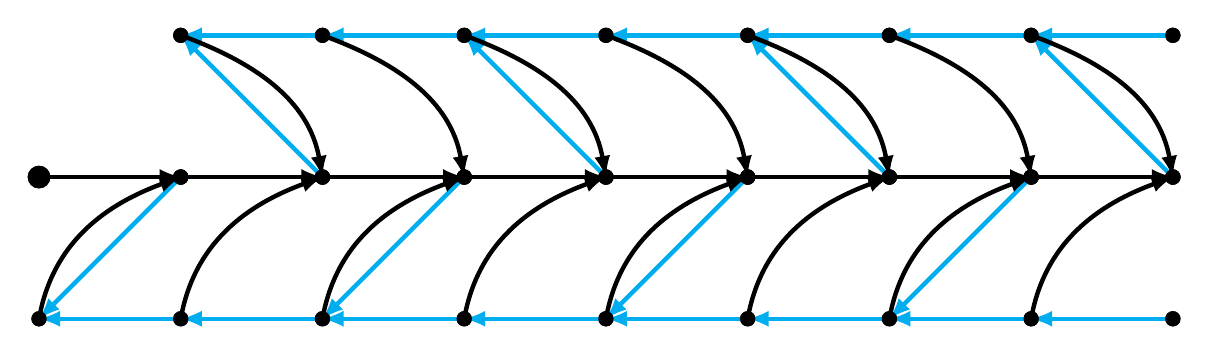
\begin{tikzpicture}[scale=1.8,main node/.style={circle,draw,font=\Large\bfseries}]
 			
 			
 			\foreach \x in {0,1,2,3,4,5,6,7,8}
 			{%
 				\draw (\x,0) circle (0.05cm);
 				\fill (\x,0) circle (0.05cm);
 				\draw (\x,-1) circle (0.05cm);
 				\fill (\x,-1) circle (0.05cm);
 			}
 			
 			\foreach \x in {1,2,3,4,5,6,7,8}
{%
	\draw (\x,0) circle (0.05cm);
	\fill (\x,0) circle (0.05cm);
	\draw (\x,1) circle (0.05cm);
	\fill (\x,1) circle (0.05cm);
}
 			
 			
 			
 			\fill (0,0) circle (0.08cm);
 			
 			
 			\foreach \x in {0,2,4,6}
 			{
 			}
 			
 			
 			
 			
 			
 			\foreach \x in {0,1,2,3,4,5,6,7}
 			{
 				\draw[ultra thick, -latex] (\x,0) to  (\x+1,0);	
\draw[ultra thick,cyan, latex-] (\x,-1) to  (\x+1,-1);	

 			}			
 			
 			\foreach \x in {1,2,3,4,5,6,7}
 			{
 				\draw[ultra thick,cyan, latex-] (\x,1) to  (\x+1,1);	
 				
 			}			
 			
 			
 			
 			 			\foreach \x in {0,2,4,6}
 			 			{ 				\draw[ultra thick,cyan, -latex] (\x+1,0) to  (\x,-1);	
 			 			}
 		 			
 		 						\foreach \x in {0,2,4,6}
 		 			{ 				\draw[ultra thick,cyan, -latex] (\x+2,0) to  (\x+1,1);	
 		 			}
 	 			
 	 			
 			\foreach \x in {0,1,2,3,4,5,6,7}
 			{
 				\draw[ultra thick, latex-] (\x+1,0)[out=200, in=80] to  (\x,-1);	
 			}
 			
 				\foreach \x in {1,2,3,4,5,6,7}
 			{
 				\draw[ultra thick, latex-] (\x+1,0)[in=-20, out=100] to  (\x,1);	
 			}
 			
 			
 			\foreach \x in {0,1,2,3,4,5,6,7,8}
 			{
 			}			
 			
 			 

 			\foreach \x in {0,1,2,3,4,5,6,7,8}
{%
	\draw (\x,0) circle (0.05cm);
	\fill (\x,0) circle (0.05cm);
	\draw (\x,-1) circle (0.05cm);
	\fill (\x,-1) circle (0.05cm);
}

\foreach \x in {1,2,3,4,5,6,7,8}
{%
	\draw (\x,0) circle (0.05cm);
	\fill (\x,0) circle (0.05cm);
	\draw (\x,1) circle (0.05cm);
	\fill (\x,1) circle (0.05cm);
}



\fill (0,0) circle (0.08cm);

 			
 			
 		\end{tikzpicture}

\end{document}